\documentclass[12pt,a4paper]{article}
\usepackage[brazilian]{babel}
\usepackage[margin=2.5cm,bottom=3cm]{geometry}
\usepackage{amsmath,amssymb,amsthm}
\usepackage{graphicx,booktabs,multirow,threeparttable}
\usepackage{csquotes}
\usepackage[authordate,backend=biber,natbib=true,doi=true,url=true,urldate=long,giveninits=false,dashed=false]{biblatex-chicago}
\addbibresource{references.bib}
\DeclareDelimFormat[bib,biblist]{finalnamedelim}{\addcomma\space\bibstring{and}\space}
\DeclareFieldFormat[online]{title}{\mkbibquote{#1\isdot}}
\usepackage{ragged2e,setspace,placeins}
 % Shared journal typography. Exporter inlines this file into each document.
% Compile with XeLaTeX; Times New Roman is also installed on Overleaf.
\usepackage{fontspec}
\setmainfont{Times New Roman}
\setsansfont{Times New Roman}
\setmonofont{Times New Roman}
\usepackage{unicode-math}
\setmathfont{TeX Gyre Termes Math}
\usepackage{setspace}
\onehalfspacing
\usepackage{etoolbox}
\usepackage{titlesec}
\titleformat{\section}{\normalfont\normalsize\itshape}{\thesection}{1em}{}
\titleformat{\subsection}{\normalfont\normalsize\itshape}{\thesubsection}{1em}{}
\titleformat{\subsubsection}{\normalfont\normalsize\itshape}{\thesubsubsection}{1em}{}
\titleformat{\paragraph}[runin]{\normalfont\normalsize\itshape}{\theparagraph}{1em}{}
\usepackage{caption}
\DeclareCaptionFont{journal}{\normalsize\onehalfspacing}
\captionsetup{font=journal,labelfont=it}
\makeatletter
% setspace resets floats to single spacing; restore journal spacing afterwards.
\AtBeginDocument{\apptocmd{\@xfloat}{\onehalfspacing\normalsize}{}{\PackageError{journal_style}{Cannot restore float spacing}{Check the float implementation.}}}
\patchcmd{\l@section}{\bfseries}{\itshape}{}{}
\patchcmd{\@footnotetext}{\reset@font\footnotesize}{\reset@font\normalsize\onehalfspacing}{}{}
\renewcommand{\footnotesize}{\normalsize}
\renewcommand{\@maketitle}{%
  \newpage\null\vskip 1.5em
  \begin{center}
    {\normalsize\itshape\@title\par}\vskip 1em
    {\normalsize\@author\par}\vskip .5em
    {\normalsize\@date\par}
  \end{center}\par\vskip 1em}
\renewenvironment{abstract}
  {\begin{center}\normalsize\itshape\abstractname\end{center}\begin{quotation}\normalsize}
  {\end{quotation}}
\makeatother
\renewcommand{\descriptionlabel}[1]{\hspace{\labelsep}\normalfont\itshape #1}
\pagestyle{plain}
\widowpenalty=10000
\clubpenalty=10000
\displaywidowpenalty=10000
\usepackage[protrusion=false]{microtype}
\usepackage{caption,xurl}
\usepackage[hidelinks]{hyperref}
% Referencia ao artigo sincronizada nesta exportacao. Se renumerar
% a tabela de resultados no main, atualize esta linha tambem.
\makeatletter
\newlabel{main-tab:mainresults}{{4}{14}{Resultados nacionais da redução a partir de 44h, com ponte horária recalibrada}{table.caption.4}{main.pdf}}
\makeatother
\graphicspath{{./}}
\onehalfspacing
\raggedbottom
\setlength{\emergencystretch}{3em}
\Urlmuskip=0mu plus 1mu\relax
\urlstyle{same}
\setcounter{topnumber}{3}
\renewcommand{\topfraction}{0.9}
\renewcommand{\textfraction}{0.08}
\renewcommand{\floatpagefraction}{0.8}
\renewcommand{\thesection}{\Alph{section}}
\renewcommand{\theequation}{A.\arabic{equation}}
\renewcommand{\thetable}{A.\arabic{table}}
\renewcommand{\thefigure}{A.\arabic{figure}}
\newcommand{\Areq}{A_{\mathrm{req}}}
\title{Apêndice online de\\[3pt]
``Jornada de trabalho, produtividade e informalidade:\\
uma avaliação quantitativa para o Brasil''}
\author{}
\date{Setembro de 2026}
\begin{document}
\maketitle
Este apêndice documenta os microdados, a correspondência entre momentos e parâmetros, a solução do modelo e as sensibilidades do artigo. O exercício principal limita as horas habituais formais da PNAD Contínua de 2024T4 a 44h na referência, recalibra a ponte de remuneração e aplica os novos tetos de 40h e 36h. Essa referência é uma hipótese de comparação. A distribuição habitual integral permanece como sensibilidade. As comparações centrais mantêm $\sigma=1{,}326$ e distinguem a atualização dos dados das correções de código.
\setcounter{tocdepth}{1}
\hypersetup{bookmarksdepth=2}
\tableofcontents
\clearpage
 \section{Dados, definições e rastreabilidade}\label{app:data}
\subsection{PNAD Contínua: período, versão e universo}
O reprocessamento utiliza os microdados públicos do quarto trimestre de 2024, arquivo \path{PNADC_042024_20250815.zip}, disponibilizado pelo IBGE, e o leiaute contido em \path{Dicionario_e_input_20221031.zip} \citep{PNAD2024T4Microdados,PNADDicionario2022}. A atualização do arquivo de pessoas é de 15 de agosto de 2025; a data do dicionário não representa a versão dos microdados. A coleta e a verificação ocorreram em 5 de setembro de 2026. As 469.334 linhas foram verificadas como pertencentes a 2024T4. Nenhum trimestre foi substituído.

A tentativa inicial de consulta à Base dos Dados via BigQuery encontrou bloqueios de autenticação e de criação de tarefas de consulta. Por isso, o processamento documentado usa os arquivos oficiais do IBGE e do Ministério do Trabalho e Emprego (MTE). Os esquemas e as consultas SQL arquivados registram a rota tentada; não são apresentados como evidência de extração pelo BigQuery. Os resultados foram calculados da fonte oficial alternativa, cuja versão e integridade podem ser verificadas.

O universo reúne pessoas com 14 anos ou mais (\texttt{V2009}), ocupadas na semana de referência (\texttt{VD4002=1}). Cada pessoa entra uma vez, com atividade, posição na ocupação, rendimento e horas do trabalho principal. O peso é \texttt{V1028}, trimestral e ajustado pela não entrevista e calibração populacional. Não se calculam médias simples dos estados nem se somam vínculos administrativos como pessoas distintas.

A amostra contém 385.717 pessoas de 14 anos ou mais e 209.311 ocupadas. Os totais ponderados são 173,430 milhões e 101,832 milhões, respectivamente; a razão entre ocupados e população de 14 anos ou mais é $0{,}587166$. A escala do modelo, $N=0{,}59$, é uma normalização mantida para preservar as unidades dos custos quadráticos. Ela não é a nova estimativa da taxa de ocupação.

\subsection{Formalidade, CNPJ e valores ausentes}
A classificação combina \texttt{VD4009} e, para empregadores e conta própria, a pergunta de CNPJ \texttt{V4019}: 1 (sim) e 2 (não). A pergunta \texttt{V4017} trata da existência de sócio trabalhando no negócio. A Tabela~\ref{tab:app_classification} explicita as categorias.
\begin{table}[htbp]
\centering
\caption{Classificação da formalidade no trabalho principal}
\label{tab:app_classification}
\normalsize
\begin{tabular}{@{}p{1.6cm}p{7.1cm}p{4.8cm}@{}}
\toprule
VD4009 & Posição na ocupação & Classificação \\
\midrule
1 e 3 & Empregado privado e doméstico com carteira & Formal \\
2 e 4 & Empregado privado e doméstico sem carteira & Informal \\
5, 6 e 7 & Empregado público com ou sem carteira, militar ou estatutário & Formal no complemento estatístico adotado \\
8 e 9 & Empregador e trabalhador por conta própria & Formal se V4019=1; informal se V4019=2 \\
10 & Trabalhador familiar auxiliar & Informal \\
Outros & Posição desconhecida, ou CNPJ desconhecido em 8/9 & Desconhecida \\
\bottomrule
\end{tabular}
\begin{minipage}{0.98\textwidth}\normalsize
\textit{Notas:} A inclusão de empregados públicos sem carteira no complemento formal segue a definição estatística adotada; não afirma regularidade jurídica de cada contrato. CNPJ ausente fora de 8/9 é não aplicável e não altera a classificação. Fonte: \citet{PNADDicionario2022}.
\end{minipage}
\end{table}

Respostas desconhecidas não são convertidas em ausência de CNPJ. O processamento registra seu peso e calcula limites inferior e superior da informalidade sobre todos os ocupados, além da taxa entre classificáveis. Nesta amostra, todos os ocupados são classificáveis, e não há peso ausente ou não positivo. A informalidade é $38{,}600087\%$. Substituir apenas \texttt{V4019} por \texttt{V4017} no mesmo arquivo gera $44{,}174116\%$; 8,951 milhões de pessoas ponderadas mudam de categoria, com erros nos dois sentidos. A comparação isola o erro de variável, não mudança temporal do mercado de trabalho.

\subsection{Horas habituais, efetivas e mapeamento da reforma}
Horas habituais do trabalho principal são \texttt{V4039}, com suporte válido de 1 a 120 horas; horas efetivas na semana de referência são \texttt{V4039C}, de 0 a 120. Zero hora efetiva é admissível. Variáveis de todos os trabalhos não substituem as do trabalho principal. A base não fornece horas contratadas para identificar diretamente exposição ao teto contratual.
\begin{table}[htbp]
\centering
\caption{Horas e rendimento: momentos nacionais de 2024T4}
\label{tab:app_hours}
\normalsize
\begin{tabular}{@{}lrrr@{}}
\toprule
Medida no trabalho principal & Total & Formal & Informal \\
\midrule
Horas habituais & 39,13169 & 41,42440 & 35,48475 \\
Horas efetivas & 37,85473 & 39,98102 & 34,47250 \\
Horas contratadas & --- & --- & --- \\
Rendimento mensal habitual (R\$) & 3.195,29 & 3.881,49 & 2.064,51 \\
\bottomrule
\end{tabular}
\begin{minipage}{0.94\textwidth}\normalsize
\textit{Notas:} V1028 é o peso. Horas cobrem todos os ocupados classificáveis; rendimentos usam renda positiva e horas habituais válidas. Rendimento é nominal, do trabalho principal (VD4016). O traço indica medida não disponível. Fonte: \citet{PNAD2024T4Microdados}.
\end{minipage}
\end{table}

Não há horas habituais ou efetivas ausentes entre ocupados. O arquivo de entrada preserva a distribuição formal completa por valor observado. Os pesos nas faixas até 36h, 37--40h e acima de 40h são $0{,}144146$, $0{,}400253$ e $0{,}455601$. Atribuir a todas as pessoas dessas faixas as jornadas de 36h, 40h e 44h seria uma aproximação adicional. A especificação principal não faz essa substituição por três pontos.

Entre os formais, $17{,}973275\%$ declaram mais de 44 horas habituais. No exercício principal, limita-se a distribuição inicial por $h_b^0=\min\{h_b,44\}$, reduzindo a média formal para $39{,}946640$h. Nos contrafactuais, $h_b(H)=\min\{h_b^0,H\}$ para $H=40$ ou $36$. Assim, a comparação é 44$\to$40/36, preservando os valores observados abaixo de 44h. A limitação inicial é hipótese de mapeamento, não observação de horas contratadas. Interpretar o corte como efeito legal é hipótese de alcance uniforme em categorias formais heterogêneas. Não se infere descumprimento legal de horas habituais acima de 44h.

Ponte e cunhas são recalibradas nesse estado inicial. A distribuição habitual integral permanece arquivada e é utilizada como sensibilidade: nessa alternativa, preservam-se todas as respostas, e o limite interno de 120h apenas reproduz o maior valor do suporte. A comparação testa o papel da cauda longa e da base inicial. Horas informais permanecem na média habitual, $h_I=35{,}484752$h, no modelo nacional.

Os pesos legados $(0{,}085,0{,}269,0{,}646)$, anteriormente atribuídos ao DIEESE como horas contratadas, não puderam ser associados a uma tabela primária verificável daquele universo e ano. Permanecem apenas nos controles antigos, como hipóteses. Não se usa publicação de outro ano para certificar retrospectivamente a atribuição.

\subsection{Rendimentos e denominadores da ponte horária}
Sejam $r_i$ o rendimento mensal habitual nominal do trabalho principal (\texttt{VD4016}), $h_i$ as horas habituais e $w_i$ o peso. Para $j\in\{F,I\}$, a amostra remunerada $\mathcal S_j$ exige renda positiva e horas válidas. A razão com horas observadas é
\begin{equation}\label{eq:app_observed_bridge}
R_h^{\mathrm{dados}}=
\frac{\left(\frac{12}{52}\sum_{i\in\mathcal S_F}w_i r_i\right)/\sum_{i\in\mathcal S_F}w_i h_i}
{\left(\frac{12}{52}\sum_{i\in\mathcal S_I}w_i r_i\right)/\sum_{i\in\mathcal S_I}w_i h_i}.
\end{equation}
O fator mensal para semanal $12/52$ cancela. Rendimento e horas de cada modalidade usam as mesmas pessoas. Um deflator comum também cancelaria; não se combinam trimestres ou conceitos diferentes.
\begin{table}[htbp]
\centering
\caption{Razões observadas de remuneração formal/informal}
\label{tab:app_wage_bridge}
\normalsize
\begin{tabular}{@{}p{7.1cm}rr@{}}
\toprule
Estimando & Ocupados pagos & Empregados privados \\
\midrule
Folha por total de horas & 1,622443 & 1,164325 \\
Rendimento semanal médio por pessoa & 1,880100 & 1,318282 \\
Médias individuais de rendimento por hora & 1,584094 & 1,174950 \\
\bottomrule
\end{tabular}
\begin{minipage}{0.96\textwidth}\normalsize
\textit{Notas:} Segunda coluna: categorias ocupacionais remuneradas; terceira: VD4009=1 ou 2. Rendimento semanal e mensal dão a mesma razão por pessoa. As três linhas são estimandos distintos. Fonte: \citet{PNAD2024T4Microdados}.
\end{minipage}
\end{table}

No exercício principal, o denominador formal usa $\min\{h_i,44\}$ nas mesmas pessoas remuneradas; rendimentos e horas informais são preservados. O alvo passa a $R_h^{44}=1{,}682473$, enquanto $R_h^{\mathrm{dados}}=1{,}622443$ permanece o momento observado da distribuição integral. Essa transformação acompanha a limitação das horas no modelo e não constitui uma nova observação de remuneração por hora contratada. Manter silenciosamente a razão integral após limitar o denominador formal mudaria o estimando da ponte.

A ponte exclui 28.603 formais e 1.381.710 informais ponderados por renda ausente ou não positiva. Há 5.006 registros amostrais de renda ausente, incluindo universos sem remuneração. O modelo abrange todos os ocupados, inclusive familiares auxiliares; estender a razão da amostra paga a esse universo é hipótese de seleção. Rendimentos de empregadores e conta própria misturam trabalho, capital e características do negócio. O momento amplo não é prêmio salarial controlado ou produtividade causal. A razão de empregados privados informa um universo restrito; transportá-la para todos os ocupados exige outra hipótese.

\subsection{RAIS, estabelecimento e participação no emprego}
A RAIS 2022 registra 52.790.864 vínculos ativos em 31/12/2022. Porte é do estabelecimento, e uma pessoa pode ter múltiplos vínculos. A planilha oficial, aba \texttt{TABELA 2}, células C87:D95, permite reconstituir a Tabela~\ref{tab:app_rais} \citep{RAIS2022TabelasVerificadas}. Não se trata de pessoas por empresas consolidadas.
\begin{table}[htbp]
\centering
\caption{Vínculos por porte de estabelecimento: RAIS 2022}
\label{tab:app_rais}
\normalsize
\begin{tabular}{@{}lr@{}}
\toprule
Porte do estabelecimento & Vínculos em 31/12/2022 \\
\midrule
1--4 & 4.747.386 \\
5--9 & 4.494.655 \\
10--19 & 5.166.304 \\
20--49 & 6.385.257 \\
\midrule
1--49 & 20.793.602 \\
Todos os portes & 52.790.864 \\
Participação de 1--49 & 39,388637\% \\
\bottomrule
\end{tabular}
\end{table}

A fonte não sustenta $59\%$ nem $13\%+19\%=32\%$ para esse recorte. As informalidades por porte de $50\%$ e $20\%$ não são observações RAIS, que cobre apenas vínculos formais. A migração ao eSocial impõe cautela temporal \citep{RAIS2022NotaTecnica}. A variável de tamanho do negócio PNAD tem universo e categorias próprios, sem correspondência automática com estabelecimento RAIS.

A correção contábil independe da escolha empírica. Para participação formal $s_{F,g}$ e informalidade $i_g$, a participação total é
\begin{equation}\label{eq:app_formal_total}
s_{N,g}=\frac{s_{F,g}/(1-i_g)}{\sum_j s_{F,j}/(1-i_j)},\qquad i=\sum_gs_{N,g}i_g.
\end{equation}
Por exemplo, $s_F=(0{,}59,0{,}41)$ e $i_g=(0{,}50,0{,}20)$ implicam $s_N=(0{,}697194,0{,}302806)$ e $i=40{,}915805\%$. $37{,}7\%$ trata participações formais como totais. O exemplo é teste contábil, não estimativa brasileira. Para evitar universos incompatíveis, o cenário nacional reprocessado usa um grupo de ocupados; os setores usam pessoas da PNAD.

\subsection{Integridade e incerteza}
A proveniência contém endereço, data, tamanho e SHA256. Os identificadores integrais são:
\begin{description}
\item[Microdados PNAD (209.873.314 bytes)]\hfill\\
{\normalsize\path{1e04e77bd7c96d212a24000e32b1f41d713ad476bc84109b72c750246f390a2a}}
\item[Dicionário (70.208 bytes)]\hfill\\
{\normalsize\path{691ce2acd94e805741c71ea699888ad628a5fb5cbf1037fdf9626eba6b99cadc}}
\item[Planilha RAIS (1.893.910 bytes)]\hfill\\
{\normalsize\path{43ec36950a6ec9598682990bf5ff5ad9bfb9b0f6ee15e1ae68de820cbc5b3684}}
\end{description}
As estimativas são pontuais, ponderadas por V1028. Não foram calculados erros-padrão com estratos e unidades primárias; as casas decimais documentam reprodução, não precisão inferencial.
 \FloatBarrier
\section{Tecnologia, calibração e solução contínua}\label{app:calibration_details}\label{app:derivations}
\subsection{Horas físicas e trabalho efetivo}\label{app:kappa_deriv}
Para o grupo $g$, sejam $\theta_{gb}$ os pesos da distribuição formal e $h_{gb}$ as horas habituais observadas. O estado inicial principal usa $H_0=44$ e $h_{gb}^0=\min\{h_{gb},44\}$; a distribuição integral é sensibilidade. Defina
\begin{align}
\bar h_{F,g}(H)&=\sum_b\theta_{gb}\min\{h_{gb},H\},\\
q_{F,g}(H)&=\sum_b\theta_{gb}\min\{h_{gb},H\}\,e\!\left(\min\{h_{gb},H\}\right),\qquad q_{I,g}=h_{I,g}e(h_{I,g}).\label{eq:app_effective_hours}
\end{align}
Horas efetivas na pesquisa e trabalho efetivo no modelo são distintos: o segundo multiplica horas físicas por eficiência tecnológica. Não se substitui a média de $he(h)$ pelo produto de médias independentes. As funções comparadas são
\begin{equation}\label{eq:app_efficiency}
e_B(h)=\exp\{-\kappa(h-h^*)^2\},\qquad e_F(h)=\exp\{-\kappa[\max\{h-h^*,0\}]^2\}.
\end{equation}
Coincidem para $h\geq h^*$; abaixo do pico, a primeira penaliza desvios e a segunda mantém eficiência unitária. O pico é da eficiência por hora, não necessariamente do produto. Como o estado inicial contém jornadas abaixo do pico e a ponte é recalibrada por função, essa coincidência não implica curvas de $\Areq$ exatamente iguais em tetos acima dele.

A elasticidade que ancora a curvatura é a de $q(h)=he(h)$:
\begin{equation}\label{eq:kappa_derivation}
\varepsilon_q=\left.\frac{d\log q(h)}{d\log h}\right|_{h=h_{\mathrm{ref}}}=1-2\kappa h_{\mathrm{ref}}(h_{\mathrm{ref}}-h^*),\quad
\kappa=\frac{1-\varepsilon_q}{2h_{\mathrm{ref}}(h_{\mathrm{ref}}-h^*)}.
\end{equation}
Na função de fadiga, exige-se $h_{\mathrm{ref}}>h^*$. Abaixo do pico, a elasticidade é um e não identifica $\kappa$. Mantêm-se as hipóteses externas $h_{\mathrm{ref}}=42{,}244$, $h^*=40$ e $\varepsilon_q=0{,}6$, resultando em $\kappa=0{,}002109804$. A referência não é a nova média PNAD. Separá-la da distribuição evita alterar silenciosamente a hipótese de eficiência. Com $\varepsilon_q=1$, impõe-se $\kappa=0$.

A literatura de horas longas motiva testar rendimentos decrescentes, mas não identifica esses parâmetros para o Brasil nem a penalidade bilateral em jornadas curtas \citep{Pencavel2015,CollewetSauermann2017}. A extrapolação à cauda longa é substantiva, como mostra a Seção~\ref{app:hours_efficiency}. $\varepsilon_q$ não é a elasticidade do produto agregado em relação às horas, que depende também da composição e dos agregadores.

\subsection{Produção, objetivo e fronteiras}
Cada grupo produz com capital fixo:
\begin{align}
Y_g&=A_gK_g^\alpha L_g^{1-\alpha},\qquad L_g=\left[\omega_g L_{F,g}^{\rho}+(1-\omega_g)L_{I,g}^{\rho}\right]^{1/\rho},\label{eq:app_production}\\
L_{F,g}&=N_{F,g}q_{F,g},\quad L_{I,g}=\eta_I N_{I,g}q_{I,g},\quad \rho=\frac{\sigma-1}{\sigma},\quad N_{I,g}=N_g-N_{F,g}.
\end{align}
O limite $\sigma=1$ é Cobb--Douglas. Para $0<\omega_g<1$ e insumos positivos, os produtos marginais por trabalhador adicional, mantendo a outra modalidade fixa, são
\begin{align}
\mathrm{MP}_{F,g}&=(1-\alpha)Y_gL_g^{-\rho}\omega_gL_{F,g}^{\rho-1}q_{F,g},\label{eq:app_mpf}\\
\mathrm{MP}_{I,g}&=(1-\alpha)Y_gL_g^{-\rho}(1-\omega_g)L_{I,g}^{\rho-1}\eta_Iq_{I,g}.\label{eq:app_mpi}
\end{align}
Têm unidades de produto semanal por trabalhador; os marginais por unidade de trabalho efetivo são outros objetos. A escolha privada contínua é
\begin{equation}\label{eq:app_objective}
\max_{0\leq x\leq N_g}J_g(x)=Y_g(x,N_g-x)-\tau_gx-\frac{\pi_g}{2}(N_g-x)^2-\frac{\gamma_g}{2}(x-\bar N_{F,g})^2.
\end{equation}
Sua condição interior é
\begin{equation}\label{eq:foc_NF}
J'_g(x)=\mathrm{MP}_{F,g}-\mathrm{MP}_{I,g}-\tau_g+\pi_g(N_g-x)-\gamma_g(x-\bar N_{F,g})=0.
\end{equation}
A diferença dos marginais é necessária porque uma unidade formal adicional retira uma informal. O termo positivo de $\pi_gN_{I,g}$ é a redução de custo informal. Não se multiplica novamente pela derivada CES após calcular $\mathrm{MP}_{F,g}$.

Para $\sigma>0$, $0<\alpha<1$, capital positivo e custos convexos não negativos, a produção composta é côncava na composição. As condições interiores e de fronteira caracterizam o máximo global. Em $x=0$, exige-se $J'_g(0^+)\leq0$; em $x=N_g$, $J'_g(N_g^-)\geq0$. O algoritmo usa limites direcionais da tecnologia, resolve a raiz interior por Brent e compara objetivos nos extremos. Proximidade numérica de um extremo não certifica otimalidade sem essas condições. Registram-se resíduo da derivada, violação de otimalidade e posição interior ou de fronteira.

\subsection{Normalização das cunhas}
O alvo de informalidade determina $\bar N_{F,g}=(1-i_g)N_g$ e $\bar N_{I,g}=i_gN_g$. No estado inicial, o custo de ajuste tem derivada zero. Com $D_g=\mathrm{MP}_{F,g}^0-\mathrm{MP}_{I,g}^0$, o momento identifica apenas
\begin{equation}\label{eq:app_wedge_identification}
\tau_g-\pi_g\bar N_{I,g}=D_g.
\end{equation}
Seleciona-se uma solução não negativa por normalização:
\begin{equation}\label{eq:app_wedge_normalization}
\tau_g\geq0,\quad\pi_g\geq0,\quad\tau_g\pi_g=0,\qquad
(\tau_g,\pi_g)=\begin{cases}(D_g,0),&D_g\geq0,\\(0,-D_g/\bar N_{I,g}),&D_g<0.\end{cases}
\end{equation}
A complementaridade separa coeficientes por convenção, sem identificação independente. Cada mudança de tecnologia ou distribuição exige recalibrar o par. Seus valores dependem das normalizações e não são alíquotas de folha ou estimativas de fiscalização. No cenário principal, $\tau_B=2{,}661015$ e $\tau_F=2{,}714237$, com $\pi=0$. Mantém-se $\gamma=0{,}06$ como hipótese.

\subsection{Ponte formal--informal e identificação condicional}\label{app:sigma_discussion}
As elasticidades de substituição dependem dos tipos de trabalho e da margem modelada. \citet{OttavianoPeri2012} estudam substituição entre nativos e imigrantes; \citet{BaharDiTellaGulek2025} examinam choques de oferta informal e permissões de trabalho. Aqui, $\sigma_{\mathrm{sub}}$ governa a substituição entre trabalho efetivo formal e informal no agregador de produção. \citet{LeyvaUrrutia2020} incorporam fricções de emprego e participação, enquanto \citet{McKiernan2021} considera a alocação de tempo das famílias entre trabalho formal, informal e produção doméstica. Essas diferenças de objeto e de estrutura impedem transportar diretamente as elasticidades entre modelos.

Mantém-se $\sigma=1{,}326$, calibrando $\omega$ condicionalmente à razão horária da Equação~\eqref{eq:app_observed_bridge}, com horas formais limitadas a 44h no alvo principal. Participação formal no emprego ou na renda não é, por identidade, peso tecnológico CES. Definindo $P_F=\sum_gN_{F,g}\mathrm{MP}_{F,g}$ e $P_I=\sum_gN_{I,g}\mathrm{MP}_{I,g}$, a ponte é
\begin{align}
R_h^{\mathrm{modelo}}&=\frac{P_F/\sum_gN_{F,g}\bar h_{F,g}}{P_I/\sum_gN_{I,g}h_{I,g}},\label{eq:app_model_bridge}\\
R_w^{\mathrm{modelo}}&=\frac{P_F/\sum_gN_{F,g}}{P_I/\sum_gN_{I,g}}.
\end{align}
Marginais são calculados por grupo antes de agregar folhas e horas. Um CES dos insumos somados não reproduz, em geral, essa agregação. A identidade $N_{F,g}\mathrm{MP}_{F,g}+N_{I,g}\mathrm{MP}_{I,g}=(1-\alpha)Y_g$ é controle de implementação.

Igualar marginais brutos a remunerações acrescenta hipótese competitiva ao problema privado com $N_g$ fixo. Esse problema isoladamente não determina salários líquidos ou distribuição de transferências. $R_h^{44}=1{,}682473$ gera $\omega_B=0{,}675651$ e $\omega_F=0{,}676650$. A razão semanal é $1{,}894029$ no modelo e $1{,}880100$ na amostra paga; o desvio $0{,}013929$ é reportado, pois ela não foi o alvo. Sua relação com as mesmas folhas e horas, além das diferenças de universo, impede interpretar proximidade como validação independente.

Uma razão não identifica conjuntamente $\sigma$, $\omega$, $\eta_I$ e cunhas. $\eta_I=0{,}40$ é hipótese de eficiência, não razão de rendimentos. Na mensuração das participações dos fatores, \citet{Gollin2002} mostra que omitir a remuneração do trabalho dos autônomos subestima a parcela do trabalho. Seus rendimentos combinam trabalho e capital. Aqui, $\alpha=0{,}35$ permanece uma hipótese, sem nova estimação dessa parcela.

\FloatBarrier
\section{Restauração do produto e recursos}\label{app:areq_resources}
\subsection{Composição reotimizada e congelada}
Para um multiplicador comum $a>0$, cada grupo resolve novamente a Equação~\eqref{eq:app_objective}, com $aA_g$. A compensação satisfaz
\begin{equation}\label{eq:app_areq}
\sum_gY_g\big(aA_g,H,N_{F,g}^*(a,H)\big)=Y_0,\qquad \Areq=a-1.
\end{equation}
A compensação é uma fração; sua expressão em porcentagem nas tabelas é $100\Areq$. A reotimização ocorre em cada avaliação da raiz e já existia no algoritmo original. O núcleo comum a preserva, verifica o intervalo da raiz e o amplia quando necessário. O erro relativo de restauração deve ser menor que $10^{-9}$.

A monotonicidade relevante é a da produção escolhida, não a de cada emprego ou insumo. Escreva a produção como $af_g(x)$ e os custos como $c_g(x)$. Se $x_1,x_2$ maximizam o objetivo em $a_1<a_2$, preferência revelada fornece
\begin{align*}
a_1f_g(x_1)-c_g(x_1)&\geq a_1f_g(x_2)-c_g(x_2),\\
a_2f_g(x_2)-c_g(x_2)&\geq a_2f_g(x_1)-c_g(x_1).
\end{align*}
Somando, $(a_2-a_1)[f_g(x_2)-f_g(x_1)]\geq0$. Portanto, $af_g(x^*(a))$ cresce estritamente onde a produção é positiva, mesmo sem monotonicidade da composição formal. Isso sustenta a raiz com custos e parâmetros fixos durante a busca.

A compensação congelada fixa o emprego no valor efetivamente obtido no estado inicial. Pela linearidade em $a$,
\begin{equation}\label{eq:app_areq_frozen}
\Areq^{\mathrm{fixa}}=\frac{Y_0}{\sum_gY_g(A_g,H,N_{F,g}^0)}-1.
\end{equation}
\begingroup\widowpenalty=10000\clubpenalty=10000
Ela não congela horas ou eficiência. Para 36h, é $7{,}955504\%$ (bilateral) e $6{,}194459\%$ (fadiga), contra $8{,}381261\%$ e $6{,}524416\%$ reotimizados. Para 40h, é $1{,}494072\%$ e $1{,}457202\%$, contra $1{,}572576\%$ e $1{,}533765\%$.
\par\endgroup

$\Areq$ tem sinal. Se a intervenção já eleva produto, reduzi-lo ao inicial pode exigir queda de $A$, gerando raiz negativa. A necessidade de ganho adicional não negativo é $\max\{\Areq,0\}$. Ambas as compensações se referem ao produto bruto, não ao consumo líquido.

\subsection{Pagamentos e fechamento}\label{app:pe_omits}
No fechamento principal, $\tau_gN_{F,g}$ e $\pi_gN_{I,g}^2/2$ são pagamentos privados devolvidos ao domicílio. O ajuste $D_g^{\mathrm{aj}}=\gamma_g(N_{F,g}-\bar N_{F,g})^2/2$ consome recursos:
\begin{equation}\label{eq:app_resources}
C^{\mathrm{ag}}+\sum_gD_g^{\mathrm{aj}}=\sum_gY_g.
\end{equation}
A opção alternativa do código destrói também os demais pagamentos:
\begin{equation}\label{eq:app_resources_alternative}
C^{\mathrm{ag}}+\sum_g\left[D_g^{\mathrm{aj}}+\tau_gN_{F,g}+\frac{\pi_g}{2}N_{I,g}^2\right]=\sum_gY_g.
\end{equation}
A mudança afeta consumo e bem-estar, sem modificar a escolha privada se seu objetivo for mantido. Não se somam transferências a custos de recursos silenciosamente.

Capital e emprego total são fixos, nacionalmente e por setor. Ficam fora do exercício a acumulação de capital, os ajustes de salários e preços, a participação na força de trabalho, a acomodação monetária e fiscal e a realocação entre setores. A partilha de trabalho é desligada pela hipótese de $N$ fixo. Não há equações de investimento, barganha ou insumo-produto. O modelo não calcula ajuste de capital em três a cinco anos nem redução numérica de $\Areq$ por esse canal. Esses mecanismos não recebem sinal ou magnitude quantitativa; omiti-los tampouco demonstra que $\Areq$ seja limite superior. Sequências de tetos são comparações estáticas ao mesmo estado inicial, não trajetórias com aprendizado ou acumulação.

\FloatBarrier
\section{Bem-estar representativo e equivalente de consumo}\label{app:welfare_additional}
Sejam $c=C^{\mathrm{ag}}/N$ o consumo por trabalhador e $h$ a média de horas físicas, ponderando emprego formal e informal. O composto GHH é
\begin{equation}\label{eq:app_ghh}
G(c,h)=c-v(h),\qquad v(h)=\frac{\psi h^{1+\nu}}{1+\nu}.
\end{equation}
Usa-se $\nu=2$ e normaliza-se $\psi$ por $\psi h_0^\nu=w_0$, com $w_0=\sum_g(1-\alpha)Y_g^0/\sum_gN_gh_g^0$ imputado pela parcela do trabalho. É uma normalização representativa, não estimativa da desutilidade na PNAD. Publicam-se
\begin{align}
\Delta GHH\;(\%)&=100\frac{G(c_1,h_1)-G(c_0,h_0)}{G(c_0,h_0)},\label{eq:app_dghh}\\
CE\;(\%)&=100\frac{c_1-c_0-v(h_1)+v(h_0)}{c_0}.\label{eq:app_ce}
\end{align}
CE satisfaz $G(c_0[1+CE/100],h_0)=G(c_1,h_1)$. Numeradores iguais com denominadores distintos não são estatísticas intercambiáveis. Denominadores inválidos são tratados como erro, não substituídos por valores arbitrários.

Em 40h, o cenário principal dá $\Delta GHH=0{,}2250\%$ e $CE=0{,}1762\%$ na bilateral; na fadiga, $0{,}2763\%$ e $0{,}2164\%$. Em 36h, a bilateral dá $-4{,}3659\%$ e $-3{,}4199\%$, e a fadiga $-2{,}1210\%$ e $-1{,}6614\%$. São resultados sem compensação de produtividade, relativamente à base formal limitada a 44h. Restaurar produto e avaliar bem-estar diferem porque horas afetam desutilidade e custos consomem recursos.

Aplica-se $v$ à média de horas, não se calcula a média de $v(h_i)$ entre pessoas heterogêneas. Não há rendas individuais, transições identificadas ou regras distributivas de lucros e transferências. Não se derivam ganhos ou perdas individuais dos que permanecem formais, passam à informalidade ou já eram informais. Composição agregada e exposição mecânica ao teto não identificam incidência. A curva representativa não identifica jornada socialmente ótima fora das hipóteses utilizadas.


\begin{figure}[htbp]
\centering
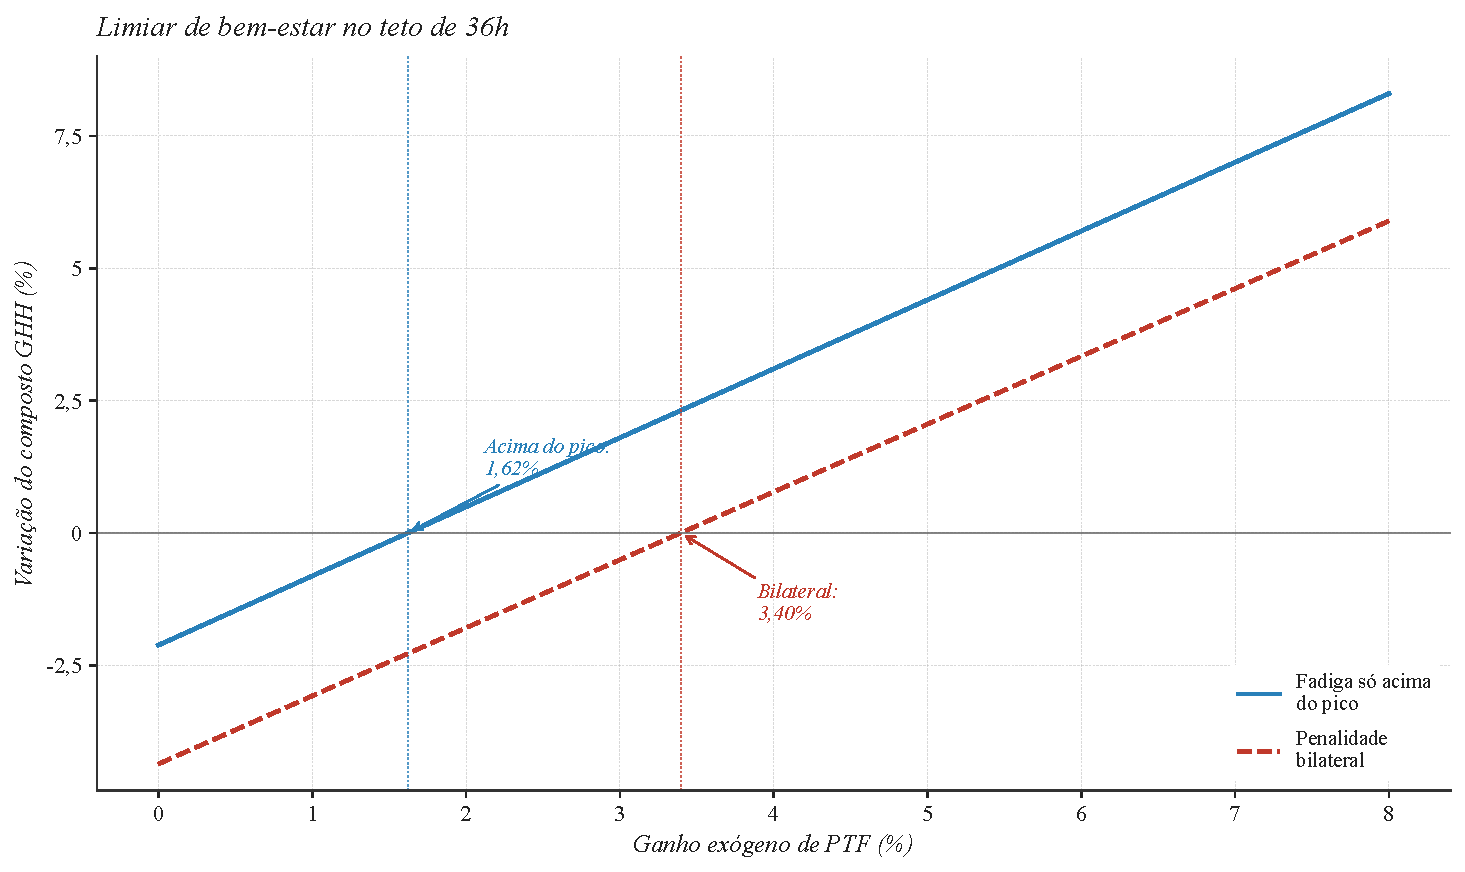
\includegraphics[width=0.95\textwidth]{slide10c_welfare_threshold.pdf}
\caption{Limiar de bem-estar no teto de 36h}\label{fig:welfare_threshold}
\begin{minipage}{0.95\textwidth}\normalsize
\textit{Notas:} Variação percentual do composto GHH em função do ganho exógeno de PTF, relativamente à base formal limitada a 44h. Composição formal--informal reotimizada em cada avaliação, preservando ponte, cunhas e preferências iniciais. O indicador cruza zero em $3{,}39647\%$ de PTF na penalidade bilateral e em $1{,}62307\%$ sob fadiga só acima do pico. CE tem o mesmo numerador e o mesmo limiar, mas denominador diferente. Curvas e verificações estão em \path{generated/welfare_threshold.csv} e \path{generated/welfare_threshold_checks.json}.
\end{minipage}
\end{figure}
 \FloatBarrier
\section{Decomposição aditiva do produto}\label{app:decomposition}
A ordem é \emph{horas físicas, eficiência e realocação formal--informal}. Seja $Y_0$ o produto inicial. O primeiro nível intermediário, $Y_H$, aplica novas horas por faixa, mantendo sua eficiência e composição iniciais. O segundo, $Y_E$, atualiza também a eficiência, preservando composição. O último, $Y_1$, permite reotimização formal--informal. $A$ mantém seu valor inicial em todos os níveis.
\begin{equation}\label{eq:app_decomposition}
\underbrace{100\frac{Y_1-Y_0}{Y_0}}_{\Delta Y}
=\underbrace{100\frac{Y_H-Y_0}{Y_0}}_{\text{horas físicas}}
+\underbrace{100\frac{Y_E-Y_H}{Y_0}}_{\text{eficiência}}
+\underbrace{100\frac{Y_1-Y_E}{Y_0}}_{\text{realocação}}.
\end{equation}
Todos os termos têm denominador comum. Interações são incorporadas à margem atualizada por último; a atribuição depende da ordem e não é única. O último termo é contrafactual definido, não resíduo com denominador diferente.
\begin{table}[htbp]
\centering
\caption{Decomposição nacional com a base formal limitada a 44h}
\label{tab:app_decomposition}
\normalsize
\begin{tabular}{@{}llrrrr@{}}
\toprule
Eficiência & Teto & Horas & Eficiência & Realocação & Total \\
\midrule
Bilateral & 40h & $-2{,}24352$ & $0{,}77145$ & $-0{,}20447$ & $-1{,}67655$ \\
Fadiga & 40h & $-2{,}18876$ & $0{,}75249$ & $-0{,}19951$ & $-1{,}63578$ \\
Bilateral & 36h & $-6{,}70703$ & $-0{,}66221$ & $-1{,}02838$ & $-8{,}39762$ \\
Fadiga & 36h & $-6{,}53974$ & $0{,}70661$ & $-0{,}81309$ & $-6{,}64622$ \\
\bottomrule
\end{tabular}
\begin{minipage}{0.96\textwidth}\normalsize
\textit{Notas:} Parcelas em pontos percentuais da variação de produto, todas divididas por $Y_0$. Valores não arredondados somam à variação total. Fadiga é eficiência constante abaixo do pico. $\sigma=1{,}326$, com ponte e cunhas recalibradas por função.
\end{minipage}
\end{table}
 % Generated by scripts/generate_assets.py; do not edit.
\begin{table}[!htbp]
\centering
\normalsize
\caption{Níveis intermediários do produto na decomposição nacional}\label{tab:decomposition_levels}
\setlength{\tabcolsep}{4pt}
\begin{tabular}{llrrrr}
\toprule
Função & Teto & $Y_0$ & $Y_H$ & $Y_E$ & $Y_1$ \\
\midrule
Bilateral & 40h & 4,184726 & 4,090841 & 4,123124 & 4,114567 \\
Bilateral & 36h & 4,184726 & 3,904055 & 3,876343 & 3,833309 \\
Acima do pico & 40h & 4,268422 & 4,174997 & 4,207116 & 4,198600 \\
Acima do pico & 36h & 4,268422 & 3,989279 & 4,019440 & 3,984733 \\
\bottomrule
\end{tabular}
\par\smallskip
\begin{minipage}{0.98\linewidth}\normalsize Fonte: simulações nacionais com PNAD 2024T4, base formal limitada a 44h e ponte horária recalibrada. Produto em unidades normalizadas do modelo, com seis casas decimais; não em reais. A ordem é horas físicas, eficiência e realocação formal--informal: $Y_H$ altera somente as horas, $Y_E$ atualiza também a eficiência, mantendo a composição inicial, e $Y_1$ permite a reotimização. As contribuições percentuais são $100(Y_H-Y_0)/Y_0$, $100(Y_E-Y_H)/Y_0$ e $100(Y_1-Y_E)/Y_0$, cuja soma é $100(Y_1-Y_0)/Y_0$. Os cálculos e o CSV usam precisão integral; diferenças aparentes após arredondamento não são resíduos econômicos.\end{minipage}
\end{table}
\begin{figure}[htbp]
\centering
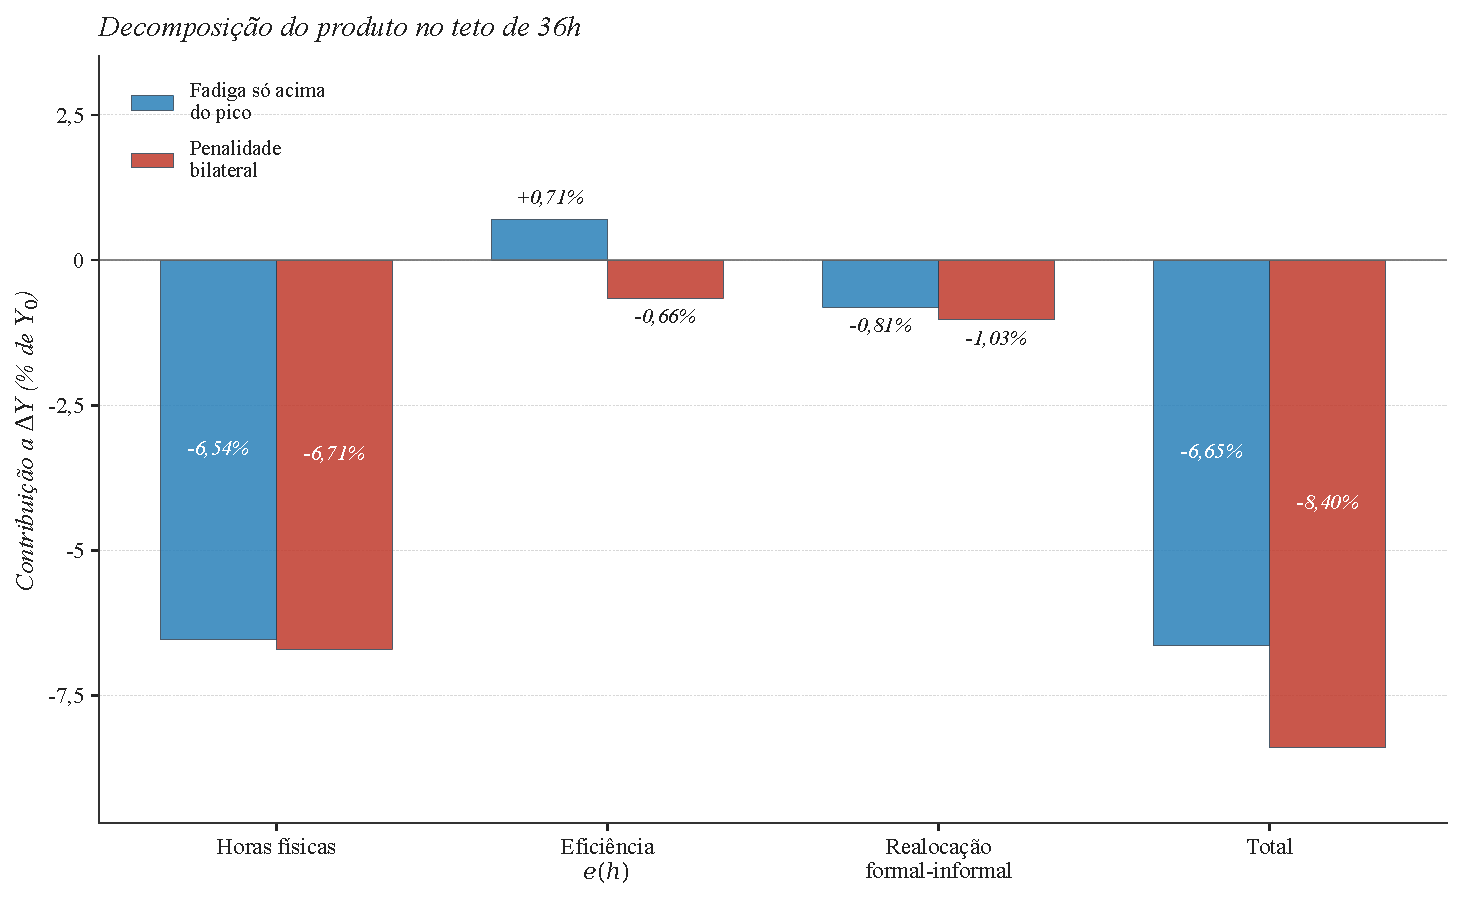
\includegraphics[width=0.96\textwidth]{fig_decomposition.pdf}
\caption{Horas físicas, eficiência e realocação na variação do produto em 36h}
\label{fig:decomposition}
\begin{minipage}{0.96\textwidth}\normalsize
\textit{Notas:} Comparação 44$\to$36h, nas duas funções de eficiência. As três parcelas usam o mesmo denominador $Y_0$ e somam à variação total, na ordem da Equação~\eqref{eq:app_decomposition}, com dados reprocessados e sem compensação exógena. Diferenças entre funções refletem também a calibração da ponte e do estado inicial.
\end{minipage}
\end{figure}

\FloatBarrier
\section{Comparação de versões e sensibilidade}\label{app:sensitivity}\label{app:hours_efficiency}
\subsection{Correções de código e atualização das entradas}
A Tabela~\ref{tab:comparison} separa execução original, núcleo corrigido com entradas congeladas e dados reprocessados. O controle congelado corrige contabilidade, resolve continuamente a composição e recalibra cunhas sob normalização explícita. Pesos de horas, taxas por porte e hipóteses legadas são preservados; isso não valida a origem empírica anteriormente atribuída a eles.

A passagem aos dados reprocessados envolve um grupo nacional e os momentos da distribuição habitual observada. Publicam-se controles intermediários: alteração isolada da participação RAIS, um grupo com entradas congeladas, $\omega=0{,}622$ com novos dados e recalibração da ponte. A versão principal limita a base formal a 44h e recalibra novamente a ponte; a distribuição integral permanece como controle de sensibilidade. Essas etapas impedem atribuir toda a diferença ao erro de CNPJ ou à otimização. Níveis de produto normalizados não devem ser comparados entre tecnologias como crescimento observado.
  % Generated by scripts/generate_assets.py; do not edit.
\begin{table}[!htbp]
\centering
\normalsize
\caption{Comparação entre versões: código e hipóteses legadas}\label{tab:comparison}
\setlength{\tabcolsep}{4pt}
\begin{tabular}{lrrrrr}
\toprule
Função e teto & $\Delta Y$ (\%) & $A_{\rm req}$ (\%) & Inf. (\%) & $\Delta GHH$ (\%) & $CE$ (\%) \\
\midrule
\addlinespace
\multicolumn{6}{l}{\textit{Original}} \\
\addlinespace
Bilateral, 40h & -2,00 & 1,92 & 38,16 & 0,41 & 0,32 \\
Bilateral, 36h & -8,02 & 8,18 & 39,62 & -3,63 & -2,84 \\
Acima do pico, 40h & -2,00 & 1,93 & 38,16 & 0,41 & 0,32 \\
Acima do pico, 36h & -6,60 & 6,63 & 39,27 & -1,76 & -1,38 \\
\addlinespace
\multicolumn{6}{l}{\textit{Código corrigido; entradas congeladas}} \\
\addlinespace
Bilateral, 40h & -2,01 & 1,92 & 41,45 & 0,23 & 0,18 \\
Bilateral, 36h & -8,07 & 8,18 & 43,14 & -4,06 & -3,18 \\
Acima do pico, 40h & -2,01 & 1,92 & 41,45 & 0,24 & 0,19 \\
Acima do pico, 36h & -6,63 & 6,62 & 42,73 & -2,17 & -1,70 \\
\addlinespace
\multicolumn{6}{l}{\textit{Ponte horária legada recalibrada}} \\
\addlinespace
Bilateral, 40h & -1,84 & 1,79 & 41,35 & 0,47 & 0,36 \\
Bilateral, 36h & -7,38 & 7,59 & 42,71 & -3,12 & -2,44 \\
Acima do pico, 40h & -1,83 & 1,79 & 41,35 & 0,47 & 0,37 \\
Acima do pico, 36h & -6,06 & 6,15 & 42,38 & -1,39 & -1,09 \\
\addlinespace
\multicolumn{6}{l}{\textit{Somente RAIS verificada}} \\
\addlinespace
Bilateral, 40h & -1,99 & 1,93 & 35,70 & 0,54 & 0,42 \\
Bilateral, 36h & -7,99 & 8,19 & 36,99 & -3,31 & -2,59 \\
Acima do pico, 40h & -1,99 & 1,92 & 35,70 & 0,54 & 0,42 \\
Acima do pico, 36h & -6,56 & 6,63 & 36,68 & -1,45 & -1,14 \\
\bottomrule
\end{tabular}
\par\smallskip
\begin{minipage}{0.98\linewidth}\normalsize Fonte: execução original arquivada e versões explicitadas da replicação corrigida. $\sigma=1{,}326$ em todas as linhas. A versão original é uma nova execução do código preservado; seu $CE$ foi calculado das alocações originais. Informalidade é nível após reforma. As versões intermediárias isolam modificações condicionais e não são todas calibrações empíricas preferidas. Na versão com RAIS, vínculos por estabelecimento são combinados apenas experimentalmente com taxas de informalidade legadas. Os conceitos e denominadores seguem a Tabela~\ref{main-tab:mainresults} do artigo.\end{minipage}
\end{table}
 % Generated by scripts/generate_assets.py; do not edit.
\begin{table}[!htbp]
\centering
\normalsize
\caption{Comparação entre versões: agregação e dados reprocessados}\label{tab:comparison_data}
\setlength{\tabcolsep}{4pt}
\begin{tabular}{lrrrrr}
\toprule
Função e teto & $\Delta Y$ (\%) & $A_{\rm req}$ (\%) & Inf. (\%) & $\Delta GHH$ (\%) & $CE$ (\%) \\
\midrule
\addlinespace
\multicolumn{6}{l}{\textit{Controle de um grupo; entradas congeladas}} \\
\addlinespace
Bilateral, 40h & -1,96 & 1,92 & 41,50 & 0,30 & 0,23 \\
Bilateral, 36h & -7,86 & 8,17 & 43,37 & -3,83 & -3,00 \\
Acima do pico, 40h & -1,96 & 1,92 & 41,50 & 0,30 & 0,24 \\
Acima do pico, 36h & -6,46 & 6,62 & 42,91 & -1,98 & -1,55 \\
\addlinespace
\multicolumn{6}{l}{\textit{PNAD reprocessada; $\omega$ fixo}} \\
\addlinespace
Bilateral, 40h & -0,07 & 0,07 & 38,62 & 3,97 & 3,11 \\
Bilateral, 36h & -6,08 & 6,26 & 40,37 & 0,05 & 0,04 \\
Acima do pico, 40h & -0,07 & 0,07 & 38,62 & 3,97 & 3,11 \\
Acima do pico, 36h & -4,54 & 4,60 & 39,90 & 2,03 & 1,59 \\
\addlinespace
\multicolumn{6}{l}{\textit{PNAD integral; sensibilidade e ponte recalibrada}} \\
\addlinespace
Bilateral, 40h & -0,08 & 0,07 & 38,63 & 3,96 & 3,10 \\
Bilateral, 36h & -6,91 & 6,80 & 40,97 & -1,01 & -0,79 \\
Acima do pico, 40h & -0,08 & 0,07 & 38,63 & 3,96 & 3,10 \\
Acima do pico, 36h & -5,17 & 5,00 & 40,35 & 1,22 & 0,96 \\
\addlinespace
\multicolumn{6}{l}{\textit{Principal: PNAD com base 44h e nova ponte}} \\
\addlinespace
Bilateral, 40h & -1,68 & 1,57 & 39,15 & 0,22 & 0,18 \\
Bilateral, 36h & -8,40 & 8,38 & 41,52 & -4,37 & -3,42 \\
Acima do pico, 40h & -1,64 & 1,53 & 39,14 & 0,28 & 0,22 \\
Acima do pico, 36h & -6,65 & 6,52 & 40,88 & -2,12 & -1,66 \\
\bottomrule
\end{tabular}
\par\smallskip
\begin{minipage}{0.98\linewidth}\normalsize Fonte: execução original arquivada e versões explicitadas da replicação corrigida. $\sigma=1{,}326$ em todas as linhas. A versão original é uma nova execução do código preservado; seu $CE$ foi calculado das alocações originais. Informalidade é nível após reforma. As versões intermediárias isolam modificações condicionais e não são todas calibrações empíricas preferidas. Na versão com RAIS, vínculos por estabelecimento são combinados apenas experimentalmente com taxas de informalidade legadas. Os conceitos e denominadores seguem a Tabela~\ref{main-tab:mainresults} do artigo.\end{minipage}
\end{table}

\subsection{Eficiência, pico e distribuição de horas}
A Tabela~\ref{tab:sensitivity} reporta exercícios condicionais com pontos interiores. Variam-se $\varepsilon_q\in\{0{,}4;0{,}6;0{,}8;1\}$, $h^*\in\{38;39;40;41\}$, $\eta_I\in\{0{,}33;0{,}40;0{,}50\}$ e $\sigma\in\{0{,}6;1;1{,}326;1{,}5;2\}$. Ponte e cunhas são recalibradas em cada ponto. Ao alterar o pico, recalcula-se a curvatura mantendo a elasticidade na referência de 42,244h: o exercício muda conjuntamente pico e curvatura sob essa âncora.
 % Generated by scripts/generate_assets.py; do not edit.
\begin{table}[!htbp]
\centering
\normalsize
\caption{Sensibilidades condicionais com a ponte horária recalibrada}\label{tab:sensitivity}
\setlength{\tabcolsep}{4pt}
\begin{tabular}{llrrrr}
\toprule
Parâmetro & Valores avaliados & Bil. 40h & Bil. 36h & Acima 40h & Acima 36h \\
\midrule
$E_Q$ & \shortstack[l]{0,4; 0,6\\0,8; 1,0} & 1,15 a 2,40 & 7,42 a 8,85 & 1,11 a 2,40 & 6,08 a 7,42 \\
$h^\star$ & \shortstack[l]{38,0; 39,0\\40,0; 41,0} & 1,50 a 1,69 & 6,55 a 11,60 & 1,48 a 1,53 & 6,25 a 6,52 \\
$\eta_I$ & 0,33; 0,40; 0,50 & 1,57 a 1,57 & 8,38 a 8,38 & 1,53 a 1,53 & 6,52 a 6,52 \\
$\sigma$ & \shortstack[l]{0,600; 1,000\\1,326; 1,500; 2,000} & 1,39 a 1,72 & 7,50 a 9,12 & 1,36 a 1,68 & 5,82 a 7,11 \\
\bottomrule
\end{tabular}
\par\smallskip
\begin{minipage}{0.98\linewidth}\normalsize Fonte: 64 simulações com PNAD 2024T4 e base formal limitada a 44h. As quatro últimas colunas mostram o mínimo e o máximo de $A_{\rm req}$ (\%) entre os valores listados; os pontos individuais estão em \texttt{generated/sensitivity\_empirical.csv}. Cada dimensão varia separadamente, incluindo pontos interiores; as demais hipóteses permanecem na base. A cada ponto, $\omega$ e as cunhas são recalibrados ao mesmo prêmio horário e à informalidade inicial. $E_Q=1$ implica ausência de fadiga. Trata-se de uma grade de sensibilidade, sem interpretação de conjunto identificado.\end{minipage}
\end{table}

A compensação depende da eficiência suposta para as jornadas. Com $\kappa=0$ e base formal limitada a 44h, $\Areq$ é $2{,}397234\%$ em 40h e $7{,}424102\%$ em 36h nas duas funções. CE é $-0{,}670986\%$ e $-2{,}520735\%$, respectivamente. Na sensibilidade com suporte integral, fadiga forte pode gerar compensação negativa em 40h. Essas diferenças impedem interpretar o número central como estimativa causal identificada de ganhos por redução de fadiga.

A distribuição integral muda a base de comparação: $\Areq$ em 40h fica entre $0{,}0721\%$ e $0{,}0739\%$, e em 36h entre $5{,}00\%$ e $6{,}80\%$, abaixo do resultado principal com limitação inicial a 44h. Mantêm-se os microdados, mas mudam transformação inicial e alvo da ponte: a razão com horas formais limitadas a 44h é $1{,}682473$, contra $1{,}622443$ na distribuição integral, com rendimento e horas informais preservados. Alterar o denominador de horas conservando silenciosamente a antiga razão não implementa o mesmo estimando.
 % Generated by scripts/generate_assets.py; do not edit.
\begin{table}[!htbp]
\centering
\normalsize
\caption{Horas de base e fadiga: compensação e equivalente de consumo}\label{tab:mapping}
\setlength{\tabcolsep}{4pt}
\begin{tabular}{llrrrr}
\toprule
Cenário & Função & $A_{\rm req}^{40}$ & $CE^{40}$ & $A_{\rm req}^{36}$ & $CE^{36}$ \\
\midrule
Principal: base 44h & Bilateral & 1,57 & 0,18 & 8,38 & -3,42 \\
Principal: base 44h & Acima do pico & 1,53 & 0,22 & 6,52 & -1,66 \\
PNAD integral & Bilateral & 0,07 & 3,10 & 6,80 & -0,79 \\
PNAD integral & Acima do pico & 0,07 & 3,10 & 5,00 & 0,96 \\
Sem fadiga (base 44h) & Bilateral & 2,40 & -0,67 & 7,42 & -2,52 \\
Sem fadiga (base 44h) & Acima do pico & 2,40 & -0,67 & 7,42 & -2,52 \\
\bottomrule
\end{tabular}
\par\smallskip
\begin{minipage}{0.98\linewidth}\normalsize Valores em \%. A limitação inicial a 44h é uma hipótese adicional de mensuração/cumprimento; altera também o denominador da ponte de remuneração horária, que é recalibrada. A base integral preserva todas as horas observadas. A ausência de fadiga mantém a base limitada a 44h e usa $E_Q=1$, $\kappa=0$. Essas alternativas não são observações distintas de horas contratuais.\end{minipage}
\end{table}

\begin{figure}[htbp]
\centering
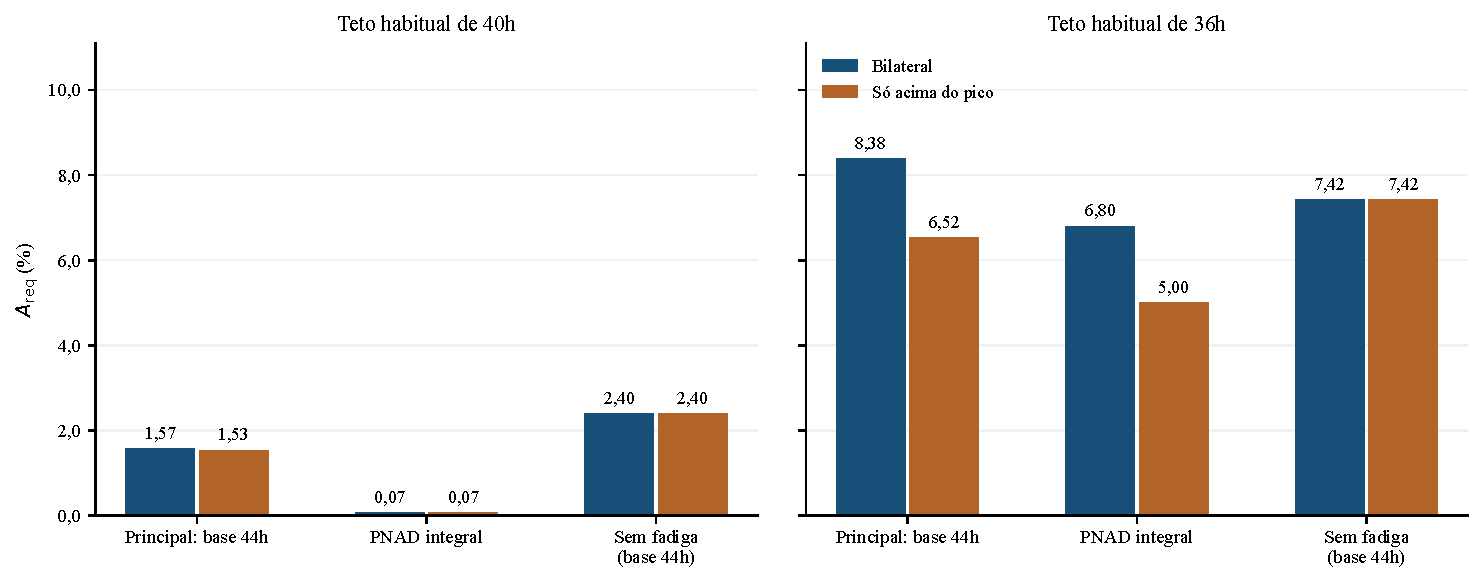
\includegraphics[width=\textwidth]{fig_sensitivity_pt.pdf}
\caption{Sensibilidade da produtividade requerida à eficiência e à distribuição inicial de horas.}\label{fig:sensitivity}
\begin{minipage}{0.96\textwidth}\normalsize
\textit{Notas:} Contrafactuais com os momentos da PNAD 2024T4, recalibrando a ponte horária e as cunhas em cada caso. A base principal limita horas formais a 44h; a distribuição integral é sensibilidade. Sem fadiga, $e(h)=1$. A Tabela~\ref{tab:sensitivity} apresenta as demais sensibilidades, incluindo pontos interiores.
\end{minipage}
\end{figure}


\subsection{CES e limites da interpretação}
Os controles congelados contêm grade conjunta de seis valores de $\sigma$, três de $\omega$ e três de $\eta_I$, além de variações de eficiência, pico e pesos de horas. A grade setorial inclui $3\times3\times3$ combinações, com vértices, faces e ponto interior. São sensibilidades. Uma caixa não é conjunto identificado: seria preciso verificar restrições empíricas em todos os pontos, incerteza amostral e correspondência entre momentos e parâmetros.

Na grade legada, o código registra se a razão horária passa pelo intervalo hipotético $[1{,}15;1{,}55]$, sem presumir que todos os pontos passem. O intervalo não se transporta automaticamente às novas razões amplas: $1{,}622443$ com horas integrais e $1{,}682473$ com horas formais limitadas a 44h, com universo e estimando explícitos. Na grade empírica, ajustar a razão com $\omega$ continua sem identificar separadamente eficiência informal e substituição. Pequena sensibilidade a um parâmetro após recalibrar outro pode refletir compensação entre eles, não precisão empírica do primeiro.

\FloatBarrier
\section{Extensão setorial}\label{app:sectoral}
\subsection{Universo e parâmetros}
A atividade do trabalho principal, CNAE Domiciliar 2.0 (\texttt{V4013}), define agropecuária nas divisões 01--03, indústria e construção em 05--43, serviços em 45--99. As 19.280 pessoas ponderadas não classificáveis são $0{,}018933\%$ dos ocupados e permanecem identificadas no arquivo. A extensão de três setores as exclui explicitamente e normaliza participações entre classificados, cobrindo $99{,}981067\%$ do emprego nacional.
\begin{table}[htbp]
\centering
\caption{Momentos setoriais reprocessados da PNAD 2024T4}
\label{tab:sectoral_params}
\normalsize
\begin{tabular}{@{}lrr@{}}
\toprule
Setor & Ocupados ponderados & Informalidade (\%) \\
\midrule
Agropecuária & 7.712.335,89 & 75,74960 \\
Indústria e construção & 20.848.824,06 & 40,25815 \\
Serviços & 73.251.518,73 & 34,21122 \\
Não classificado & 19.279,83 & 60,02732 \\
\bottomrule
\end{tabular}
\begin{minipage}{0.95\textwidth}\normalsize
\textit{Notas:} Ocupados de 14 anos ou mais, peso V1028. Formalidade usa VD4009 e V4019. As contagens preservam o universo observado; no exercício principal de cada setor, limitam-se as horas habituais formais a 44h antes da calibração. Fonte: \citet{PNAD2024T4Microdados}.
\end{minipage}
\end{table}

Cada setor contém um grupo representativo com emprego e capital fixos. Os pesos de capital $(0{,}0766;0{,}2585;0{,}6649)$ são hipóteses herdadas, originalmente atribuídas a participações de VAB. Mesmo que VAB fosse observado, sua igualdade à participação no capital exigiria outra hipótese. Com $A_g=1$, a composição de produto não é VAB observado. Mantêm-se $\alpha=0{,}35$, $\eta_I=0{,}40$, $\sigma=1{,}326$, $\gamma_g=0{,}06$ e a mesma âncora externa de eficiência.

Calibra-se $\omega$ comum somando folhas e horas dos três setores classificados antes da razão. Com horas formais limitadas a 44h, o alvo é $1{,}682335$, ligeiramente distinto do nacional, $1{,}682473$, pela exclusão das atividades não classificadas também na amostra remunerada. A raiz é $0{,}674476$ na bilateral e $0{,}675575$ na fadiga, distinta da raiz de um grupo. Recalibra-se cada cunha à informalidade setorial. A versão integral com $\omega=0{,}622$ permanece como controle.

\subsection{Resultados e agregação}
 % Generated by scripts/generate_assets.py; do not edit.
\begin{table}[!htbp]
\centering
\normalsize
\caption{Resultados setoriais com momentos da PNAD 2024T4}\label{tab:sectoral_results}
\setlength{\tabcolsep}{4pt}
\begin{tabular}{lrrrrrr}
\toprule
Setor & $\Delta Y$ & $A_{\rm req}$ & $A_{\rm req}^{fixo}$ & $\Delta$ Inf. & $\Delta GHH$ & $CE$ \\
\midrule
\addlinespace
\multicolumn{7}{l}{\textit{Bilateral, teto de 40h}} \\
\addlinespace
Agropecuária & -3,08 & 2,09 & 1,90 & 0,82 & -2,44 & -1,91 \\
Indústria e construção & -1,88 & 1,75 & 1,65 & 0,64 & 0,18 & 0,14 \\
Serviços & -1,54 & 1,50 & 1,44 & 0,44 & 0,42 & 0,33 \\
Agregado & -1,71 & 1,60 & 1,51 & 0,51 & 0,18 & 0,14 \\
\addlinespace
\multicolumn{7}{l}{\textit{Bilateral, teto de 36h}} \\
\addlinespace
Agropecuária & -12,06 & 8,85 & 8,03 & 3,21 & -12,06 & -9,44 \\
Indústria e construção & -9,05 & 8,97 & 8,48 & 3,27 & -4,90 & -3,84 \\
Serviços & -7,92 & 8,16 & 7,84 & 2,39 & -3,54 & -2,77 \\
Agregado & -8,42 & 8,41 & 8,00 & 2,63 & -4,39 & -3,44 \\
\addlinespace
\multicolumn{7}{l}{\textit{Só acima do pico, teto de 40h}} \\
\addlinespace
Agropecuária & -3,05 & 2,06 & 1,88 & 0,81 & -2,40 & -1,88 \\
Indústria e construção & -1,87 & 1,73 & 1,64 & 0,64 & 0,20 & 0,15 \\
Serviços & -1,50 & 1,45 & 1,39 & 0,42 & 0,48 & 0,37 \\
Agregado & -1,67 & 1,56 & 1,48 & 0,50 & 0,23 & 0,18 \\
\addlinespace
\multicolumn{7}{l}{\textit{Só acima do pico, teto de 36h}} \\
\addlinespace
Agropecuária & -9,88 & 7,10 & 6,44 & 2,63 & -9,26 & -7,25 \\
Indústria e construção & -7,31 & 7,12 & 6,74 & 2,61 & -2,66 & -2,09 \\
Serviços & -6,22 & 6,31 & 6,06 & 1,84 & -1,37 & -1,07 \\
Agregado & -6,68 & 6,56 & 6,24 & 2,06 & -2,16 & -1,69 \\
\bottomrule
\end{tabular}
\par\smallskip
\begin{minipage}{0.98\linewidth}\normalsize Fonte: PNAD 2024T4 reprocessada; todas as colunas em \%, exceto informalidade em pontos percentuais. Base formal limitada a 44h; horas informais preservadas. O capital setorial e os parâmetros tecnológicos são hipóteses; $\sigma=1{,}326$. A ponte soma folhas e horas entre os três setores classificados, com horas formais limitadas a 44h e $\omega=0,674476$ (bilateral) e $0,675575$ (acima). O agregado recompõe a soma dos produtos com multiplicador comum de produtividade; não é a média dos $A_{\rm req}$ setoriais. Os 0,019\% de ocupados sem atividade classificável são excluídos e as participações são renormalizadas. Capital e ocupação setoriais são fixos; os resultados não incorporam relações insumo-produto.\end{minipage}
\end{table}
O agregado soma produtos e resolve a restauração com produtividade comum, reotimizando as três composições. Sua compensação não é a média simples das setoriais. A heterogeneidade de horas, emprego, capital e eficiência impede exigir coincidência com o modelo nacional de um grupo.

Para 40h, $\Areq$ bilateral é $2{,}0854\%$ na agropecuária, $1{,}7461\%$ na indústria e $1{,}4951\%$ nos serviços; agregadamente, $1{,}6015\%$. Para 36h, é $8{,}8540\%$, $8{,}9691\%$ e $8{,}1616\%$, com agregado $8{,}4051\%$. Na fadiga, em 36h, é $7{,}1044\%$, $7{,}1235\%$ e $6{,}3090\%$, com agregado $6{,}5600\%$. Todos esses resultados comparam o novo teto à base formal limitada a 44h.
\begin{figure}[htbp]
\centering
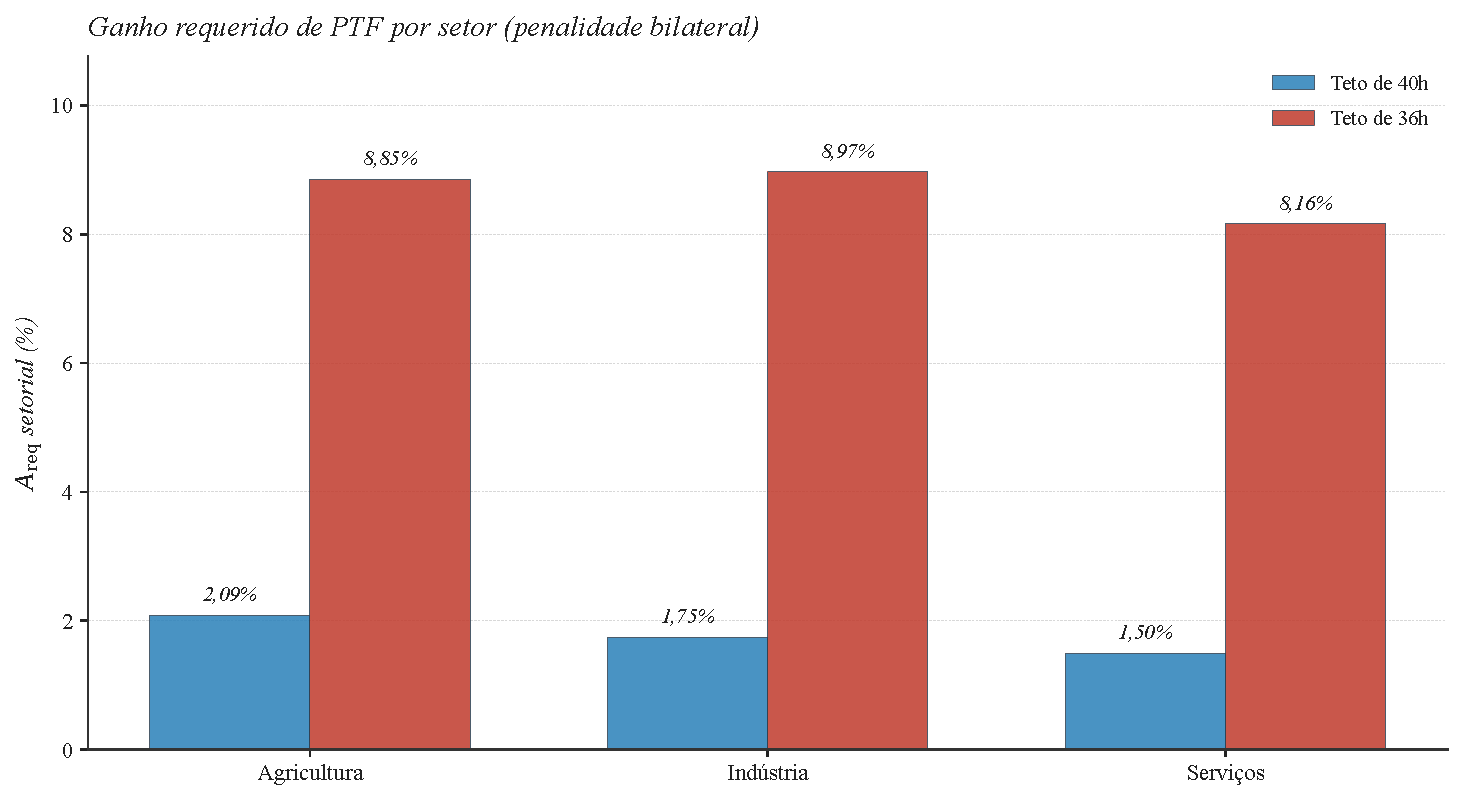
\includegraphics[width=0.96\textwidth]{fig_sectoral_areq.pdf}
\caption{Compensação de produtividade por setor nos tetos de 40h e 36h}
\label{fig:sectoral_areq}
\begin{minipage}{0.96\textwidth}\normalsize
\textit{Notas:} Penalidade bilateral, PNAD 2024T4 reprocessada, base formal limitada a 44h, $\sigma=1{,}326$ e ponte agregada recalibrada. Compensação com sinal e reotimização por setor. A Tabela~\ref{tab:sectoral_results} apresenta também a outra função e o agregado, cuja raiz é resolvida conjuntamente.
\end{minipage}
\end{figure}

Diferenças setoriais não identificam efeitos causais ou política ótima de exceções. Não há mobilidade intersetorial, insumo-produto ou heterogeneidade simultânea por porte e setor. Contagens acima do teto medem exposição mecânica nas horas habituais; não identificam emprego criado, perda individual ou incidência de bem-estar.

\FloatBarrier
\section{Produtividade histórica e horizontes}\label{app:tfp_history_table}
A série brasileira \texttt{rtfpna} da PWT 11.0, arquivada pela série FRED \texttt{RTFPNABRA632NRUG}, fornece referência de escala \citep{PWT2025,FREDPWTBrazil2026}. Usam-se taxas geométricas entre anos disponíveis. Para ganho cumulativo $a-1=\Areq$, expresso como fração, a taxa anual constante equivalente em $T$ anos é
\begin{equation}\label{eq:app_annualized}
g_T=100\left[(1+\Areq)^{1/T}-1\right].
\end{equation}
Ela não é $100\Areq/T$ exceto aproximadamente para pequenas variações. A Tabela~\ref{tab:tfp_horizons} aplica a transformação aos resultados atuais e declara o período histórico.
 % Generated by scripts/generate_assets.py; do not edit.
\begin{table}[!htbp]
\centering
\normalsize
\caption{Anualização contábil da compensação de produtividade}\label{tab:tfp_horizons}
\setlength{\tabcolsep}{4pt}
\begin{tabular}{llrrrr}
\toprule
Função & Teto & $A_{\rm req}$ (\%) & 3 anos & 5 anos & 10 anos \\
\midrule
Bilateral & 40h & 1,573 & 0,521 & 0,313 & 0,156 \\
Bilateral & 36h & 8,381 & 2,719 & 1,623 & 0,808 \\
Acima do pico & 40h & 1,534 & 0,509 & 0,305 & 0,152 \\
Acima do pico & 36h & 6,524 & 2,129 & 1,272 & 0,634 \\
\bottomrule
\end{tabular}
\par\smallskip
\begin{minipage}{0.98\linewidth}\normalsize Os ganhos anuais em \% são $g_T=100[(1+A_{\rm req})^{1/T}-1]$, com $A_{\rm req}$ em fração. Base: horas formais limitadas a 44h. A anualização apenas expressa a mesma diferença de nível em outra escala; não é uma trajetória dinâmica estimada. Na PWT 11.0 via FRED, o crescimento anualizado de produtividade do Brasil foi -0,83\% em 1990--2023. Entre janelas de dez anos inteiramente contidas em 1990--2019, a maior taxa foi 0,05\% em 2000--2010. A série serve como referência descritiva de escala e não valida o contrafactual.\end{minipage}
\end{table}

Anualização torna escalas comparáveis; não fornece trajetória de produtividade, nem atribui crescimento à reforma ou garante disponibilidade causal do ganho histórico para financiá-la. Tampouco converte o modelo estático em previsão para três, cinco ou dez anos. A referência PWT difere do canal $e(h)$: somar o mesmo ganho à produtividade exógena e ao trabalho efetivo contaria duas vezes o mecanismo.

\FloatBarrier
\section{Verificação numérica e reprodução}\label{app:replication}
Os dados, controles e resultados nacionais com base limitada a 44h provêm da execução \path{20260905_005724_846373}, concluída integralmente. O pacote registra comandos, versões, entradas, parâmetros, logs e hashes. Código e resultados anteriores foram arquivados antes das alterações. A execução original em saída vazia encontrou uma dependência setorial não gerada pelo antigo orquestrador; as simulações originais do comparativo foram reexecutadas com código arquivado, em processo separado. Figuras antigas não foram consideradas evidência de reprodução.

A reprodução integrada usa, a partir de \path{replication_package}:
\begin{quote}\normalsize
\verb|python run_all.py --refresh-data --tests --paper|
\end{quote}
A reconstrução documental usa \texttt{python build\_paper.py}, a partir de \path{PAPER}. O comando lê arquivos verificados dessa execução e recalcula os exercícios setoriais, a sensibilidade com base limitada a 44h e as curvas adicionais pelo núcleo comum. Também regenera tabelas e figuras e compila os documentos, registrando origens, parâmetros e verificações em \path{generated/ASSET_MANIFEST.json}. As distribuições integrais permanecem nos arquivos de sensibilidade e nos controles de comparação.

Os 61 testes do pacote verificam conversão formal/total, dados e pesos, limites CES, condições de primeira ordem, otimizador independente, cunhas, ponte, restauração, composição congelada, decomposição, recursos e definição de CE. A auditoria da execução de referência verificou 195 hashes e 48 simulações com 264 alocações: maior erro relativo de restauração $2{,}14\times10^{-13}$; maior discrepância de decomposição $5{,}33\times10^{-15}$ pontos percentuais. Nos 80 exercícios adicionais com base limitada a 44h, os maiores erros são $7{,}11\times10^{-15}$ na restauração e $1{,}78\times10^{-15}$ pontos percentuais na decomposição; as âncoras nacionais reproduzem o arquivo canônico.

São controles computacionais e contábeis. Recuperar pesos, médias de horas e taxas usados na calibração não é validação comportamental externa. Resultados dependem de eficiência, remuneração competitiva, recursos, preferências e alcance do teto. Evidências de outras reformas contextualizam mecanismos, mas não identificam automaticamente os parâmetros nem eliminam limitações de universo e mensuração.
\clearpage
\printbibliography
\end{document}
